\RequirePackage{ifpdf}

%\documentclass[a4paper,11pt]{scrartcl} % scrartcl scrreprt
\documentclass[a4paper,11pt]{scrartcl} % scrartcl scrreprt

\usepackage[margin=2.cm]{geometry}
\usepackage{multirow}
\usepackage{tabularx} 
\usepackage{appendix} 

\ifpdf
  \usepackage[pdftex]{graphicx}
\else
  \usepackage[dvips]{graphicx}
\fi

%\usepackage[utf8]{inputenc}
\usepackage[T1]{fontenc}

\usepackage{amsmath}
\usepackage[amssymb]{SIunits}
\usepackage{hyperref}

\usepackage{lineno}
\linenumbers

\usepackage{xcolor}

%
% DOCUMENT STARTS HERE
%
% $Id: commands.tex 909 2013-06-03 14:10:59Z rpreghen $
% Adaptation of a file originally by Roberto Preghenella (thanks!) 
%==========================================================%
\newcommand{\btwo}{\ensuremath{B_{2}}}
\newcommand{\bthree}{\ensuremath{B_{3}}}
\newcommand{\bA}{\ensuremath{B_{A}}}
\newcommand{\bthreeLambda}{$B_{3, \Lambda}$}

%nuclei and hypernuclei
\newcommand{\tritium}{\ensuremath{{}^{3}\mathrm{H}}}
\newcommand{\hethree}{\ensuremath{{}^{3}\mathrm{He}}}
\newcommand{\hefour}{\ensuremath{{}^{4}\mathrm{He}}}
\newcommand{\hthreelambda}{\ensuremath{{}^{3}_{\Lambda}\mathrm{H}}}
\newcommand{\hfourlambda}{\ensuremath{{}^{4}_{\Lambda}\mathrm{H}}}
\newcommand{\hfourtwolambda}{\ensuremath{{}^{4}_{\Lambda\Lambda}\mathrm{H}}}
\newcommand{\hefourlambda}{\ensuremath{{}^{4}_{\Lambda}\mathrm{He}}}

\newcommand{\antitritium}{\ensuremath{{}^{3}\overline{\mathrm{He}}}}
\newcommand{\antihethree}{\ensuremath{{}^{3}\overline{\mathrm{He}}}}
\newcommand{\antihefour}{\ensuremath{${}^{4}$\overline{\mathrm{He}}}}
\newcommand{\antihthreelambda}{\ensuremath{{}^{3}_{\Lambda}\overline{\mathrm{He}}}}
\newcommand{\antihfourlambda}{\ensuremath{{}^{4}_{\Lambda}\overline{\mathrm{H}}}}
\newcommand{\antihefourlambda}{\ensuremath{{}^{4}_{\Lambda}\overline{\mathrm{He}}}}
\newcommand{\antihfourtwolambda}{\ensuremath{{}^{4}_{\Lambda\Lambda}\overline{\mathrm{H}}}}

\newcommand{\dradius}{\ensuremath{r_{d}}}
\newcommand{\rperp}{\ensuremath{R_{\perp}}}
\newcommand{\rpar}{\ensuremath{R_{\|}}}



%==========================================================%
\newcommand{\Om}{$\Omega^-$}
\newcommand{\Mo}{$\overline{\Omega}^+$}
\newcommand{\X}{$\Xi^-$}
\newcommand{\Ix}{$\overline{\Xi}^+$}
\newcommand{\Xis}{$\Xi^{\pm}$}
\newcommand{\Oms}{$\Omega^{\pm}$}
\newcommand{\meanpt}{$\langle p_\mathrm{t}\rangle$}
\newcommand{\nineH}{$\sqrt{s}~=~0.9$~TeV}
\newcommand{\seven}{$\sqrt{s}~=~7$~TeV}
\newcommand{\twoH}{$\sqrt{s}~=~0.2$~TeV}
\newcommand{\dndy}{d$N$/d$y$}
\newcommand{\LT}{L{\'e}vy-Tsallis}
\newcommand{\GeVc}{GeV/$c$}
\newcommand{\MeVc}{MeV/$c$}
\newcommand{\GeVcs}{GeV/$c$ }
\newcommand{\MeVcs}{MeV/$c$ }
\newcommand{\GeVmass}{GeV/$c^2$}
\newcommand{\MeVmass}{MeV/$c^2$}
\newcommand{\allpart}{\kzero, \lmb, \almb, \X, \Ix, \Om and \Mo}

\newcommand{\ITS}          {\rm{ITS }}
\newcommand{\TOF}          {\rm{TOF }}
\newcommand{\ZDC}          {\rm{ZDC }}
\newcommand{\ZDCs}         {\rm{ZDCs }}
\newcommand{\ZNA}          {\rm{ZNA }}
\newcommand{\ZNC}          {\rm{ZNC }}
\newcommand{\SPD}          {\rm{SPD }}
\newcommand{\SDD}          {\rm{SDD }}
\newcommand{\SSD}          {\rm{SSD }}
\newcommand{\TPC}          {\rm{TPC }}
\newcommand{\VZERO}        {\rm{VZERO }}
\newcommand{\VZEROA}       {\rm{VZERO-A }}
\newcommand{\VZEROC}       {\rm{VZERO-C }}
\newcommand{\pip}          {\ensuremath{\pi^{+}}}
\newcommand{\pim}          {\ensuremath{\pi^{-}}}
\newcommand{\pipm}          {\ensuremath{\pi^{\pm}}}
\newcommand{\kap}          {\ensuremath{\mathrm{K}^{+}}}
\newcommand{\kam}          {\ensuremath{\mathrm{K}^{-}}}
\newcommand{\kapm}          {\ensuremath{\mathrm{K}^{\pm}}}
\newcommand{\p}               {$\rm p$}
\newcommand{\pbar}         {$\rm\overline{p}$}
\newcommand{\kzero}        {\ensuremath{{\rm K}^{0}_{S}}}
\newcommand{\kstar}        {\ensuremath{{\rm K}^{*0}}}
\newcommand{\lmb}          {\ensuremath{\Lambda}}
\newcommand{\almb}         {\ensuremath{\overline{\Lambda}}}
%this is another analysis...
%\newcommand{\allpart}      {$\pi^{\pm}$, K$^{\pm}$, \kzero, p(\pbar) and \lmb(\almb)}
%\newcommand{\degree}       {$^{\rm o}$}
\newcommand{\dg}           {\mbox{$^\circ$}}
\newcommand{\dedx}         {\ensuremath{\mathrm{d}E/\mathrm{d}x}}
\newcommand{\pp}           {pp}
\newcommand{\ppbar}        {\mbox{$\mathrm {p\overline{p}}$}}
\newcommand{\PbPb}         {\mbox{Pb--Pb}}
\newcommand{\pPb}          {\mbox{p--Pb}}
\newcommand{\AuAu}         {\mbox{Au--Au}}
\newcommand{\pseudorap}    {\mbox{$\left | \eta \right | $}}
\newcommand{\dNdeta}       {\ensuremath{\mathrm{d}N_\mathrm{ch}/\mathrm{d}\eta}}

\newcommand{\avdNdeta}       {\ensuremath{\left<\mathrm{d}N_\mathrm{ch}/\mathrm{d}\eta\right>}}
\newcommand{\dNchdy}         {\ensuremath{\mathrm{d}N_\mathrm{ch}/\mathrm{d}y}}
\newcommand{\dNdy}         {\ensuremath{\mathrm{d}N/\mathrm{d}y} }
\newcommand{\dNdyst}       {\ensuremath{\sqrt{\frac{dN_\pi/dy}{s_T}}}}
\newcommand{\dNdetatr}     {\mathrm{d}N_\mathrm{tracklets}/\mathrm{d}\eta}
\newcommand{\dNdetar}[1]   {\mathrm{d}N_\mathrm{ch}/\mathrm{d}\eta\left.\right|_{|\eta|<#1}}
\newcommand{\lum}          {\, \mbox{${\rm cm}^{-2} {\rm s}^{-1}$}}
%\newcommand{\barn}         {\, \mbox{${\rm barn}$}}
\newcommand{\m}            {\, \mbox{${\rm m}$}}
\newcommand{\ncls}         {\ensuremath{N_{cls}}}
\newcommand{\nsigma}       {\ensuremath{n\sigma}}
\newcommand{\dcaxy}        {\ensuremath{{\rm DCA}_{xy}} }
\newcommand{\dcaz}         {\ensuremath{{\rm DCA}_{z}} }
\newcommand{\EcrossB}      {E$\times$B}%{\ensuremath{{\rm E}\times{\rm B}}}
\newcommand{\bb}           {Bethe-Bloch}
\newcommand{\s}            {\ensuremath{\sqrt{s}}}
\newcommand{\pt}           {\ensuremath{p_{\mathrm{T}}}}
\newcommand{\pts}           {\ensuremath{p_{\rm T}} }
\newcommand{\hlab}         {\ensuremath{\eta_{\rm lab}}}
\newcommand{\ynn}         {\ensuremath{y_{\rm NN}}}
\newcommand{\ycms}         {\ensuremath{y_{\rm CMS}}}
\newcommand{\ylab}         {\ensuremath{y_{\rm lab}}}
\newcommand{\ppi}          {\ensuremath{{\rm p}/\pi}}
\newcommand{\kpi}          {\ensuremath{{\rm K}/\pi}}
\newcommand{\lpi}          {\ensuremath{{\rm \Lambda}/\pi}}
%\newcommand{\ppi}          {\ensuremath{(\pi^+ + \pi^-)/({\rm K}^+ + {\rm K}^-)}}
%\newcommand{\kpi}          {\ensuremath{({\rm p} + {\rm \bar p})/({\rm K}^+ + {\rm K}^-)}}
\newcommand{\mt}           {\ensuremath{m_{\rm T}}}
\newcommand{\snn}          {\ensuremath{\sqrt{s_{\rm NN}}}}
\newcommand{\snnbf}        {\ensuremath{\mathbf{{\sqrt{s_{\mathbf NN}}}}}}
\newcommand{\sonly}        {\ensuremath{\sqrt{s}}}
\newcommand{\Npart}        {\ensuremath{N_\mathrm{part}}}
\newcommand{\avNpart}      {\ensuremath{\langle N_\mathrm{part} \rangle}}
\newcommand{\avNpartdata}  {\ensuremath{\langle N_\mathrm{part}^{\rm data} \rangle}}
\newcommand{\Ncoll}        {\ensuremath{N_\mathrm{coll}}}
\newcommand{\Dnpart}       {\ensuremath{D\left(\Npart\right)}}
\newcommand{\DnpartExp}    {\ensuremath{D_{\rm exp}\left(\Npart\right)}}
\newcommand{\dNdetapt}     {\ensuremath{\dNdeta\,/\left(0.5\Npart\right)}}
\newcommand{\dNdetaptr}[1] {\ensuremath{\dNdetar{#1}\,/\left(0.5\Npart\right)}}
\newcommand{\dNdetape}     {\left(\ensuremath{\dNdeta\right)/\left(\avNpart/2\right)}}
\newcommand{\dNdetaper}[1] {\ensuremath{\dNdetar{#1}\,/\left(\avNpart/2\right)}}
\newcommand{\dndydpt}      {\ensuremath{{\rm d}^2N/({\rm d}y {\rm d}p_{\rm t})}}
\newcommand{\abs}[1]       {\ensuremath{\left|#1\right|}}
\newcommand{\signn}        {\ensuremath{\sigma^{\rm inel.}_{\rm NN}}}
\newcommand{\vz}           {\ensuremath{V_{z}}}
\newcommand{\Tfo}          {\ensuremath{{T}_{\rm kin}}}
\newcommand{\Tch}          {\ensuremath{{T}_{\rm ch}}}
\newcommand{\bT}           {\ensuremath{\beta_{\rm T}}}
\newcommand{\avbT}         {\ensuremath{\left< \beta_{\rm T}\right>}}
\newcommand{\avpT}         {\ensuremath{\left< \pt \right>}\xspace}
\newcommand{\muB}          {\ensuremath{\mu_{B}}}
\newcommand{\stat}         {({\it stat.})}
\newcommand{\syst}         {({\it sys.})}
\newcommand{\Fig}[1]       {Fig.~\ref{#1}}
\newcommand{\Figure}[1]    {Figure~\ref{#1}}
\newcommand{\Ref}[1]       {Ref.~\cite{#1}}
\newcommand{\green}[1]     {\textcolor{green}{#1}}
\newcommand{\blue}[1]      {\textcolor{blue}{#1}}
\newcommand{\red}[1]       {\textcolor{red}{#1}}
\newcommand{\white}[1]     {\textcolor{white}{#1}}
\newcommand{\gevc}         {\ensuremath{{\rm GeV}/c}}
\newcommand{\mevc}         {\ensuremath{{\rm MeV}/c}}
\newcommand{\gevcs}         {\ensuremath{{\rm GeV}/c} }
\newcommand{\mevcs}         {\ensuremath{{\rm MeV}/c} }
\newcommand{\avg}[1]       {\ensuremath{\left\langle#1\right\rangle}}

\newcommand {\dEdx}      {d\textit{E}/d\textit{x}\xspace}
\newcommand {\Zvtx}   {\ensuremath{Z_\mathrm{vtx}}\xspace}
\newcommand {\pT}   {\pt}

\newcommand {\proton}     		{\ensuremath{p}}
\newcommand {\electron}   		{\Pe}
\newcommand {\pion}    	  		{\ensuremath{\pi}}
\newcommand {\kaon}       		{\ensuremath{K}}
\newcommand {\KTopi}      		{\kaon/\pion}
\newcommand {\pTopi}      		{\proton/\pion}
\newcommand {\KzeroShort} 		{\PKzS}
\newcommand {\lambdaBaryon} 	{\PGL}
\newcommand {\antiLambdaBaryon} {\PAGL}
\newcommand {\gammaPhoton} 		{\PGg}
\newcommand {\Nevt}      {\ensuremath{N_\mathrm{evt}}\xspace}
\newcommand {\NevtMB}  {\ensuremath{N_\mathrm{evt|MB}}\xspace}
\newcommand {\NevtMBVTX}  {\ensuremath{N_\mathrm{evt|(MB\, \&\, Vtx)}}\xspace}
\newcommand {\NevtMBVTXZ}  {\ensuremath{N_\mathrm{evt|(MB\, \& Vtx\, \&\, \textit{Z}_{vtx})}}\xspace}
\newcommand {\NevtINEL}  {\ensuremath{N_\mathrm{evt}(\textsc{inel})}\xspace}
\newcommand {\fPrim}       {\ensuremath{f_{\mathrm{prim}}}\xspace}
\newcommand {\NPrim}     {\ensuremath{N_{\mathrm{prim}}}\xspace}
\newcommand {\NSec}      {\ensuremath{N_{\mathrm{sec}}}\xspace}
\newcommand {\NPrimTilde}     {\ensuremath{\widetilde{N}_{\mathrm{prim}}}\xspace}
\newcommand {\NSecTilde}      {\ensuremath{\widetilde{N}_{\mathrm{sec}}}\xspace}
\newcommand {\NTilde}      {\ensuremath{\widetilde{N}}\xspace}

\newcommand{\pPiplus}{\ensuremath{{\pi}^{+}}\xspace}
\newcommand{\pPiminus}{\ensuremath{{\pi}^{-}}\xspace}
\newcommand{\sPi}{\ensuremath{{\pi}}\xspace}
\newcommand{\pKplus}{\ensuremath{{\rm K}^{+}}\xspace}
\newcommand{\pKminus}{\ensuremath{{\rm K}^{-}}\xspace}
\newcommand{\sProton}{\ensuremath{\rm p}\xspace}
\newcommand{\pProton}{\ensuremath{\rm p}\xspace}
\newcommand{\apProton}{\ensuremath{\overline{\rm p}}\xspace}
\newcommand{\sPr}{\ensuremath{\rm p}\xspace}
\newcommand{\sKzero}{\ensuremath{2{\rm K}^{0}_{S}}\xspace}
\newcommand{\pKzero}{\ensuremath{{\rm K}^{0}_{S}}\xspace}
\newcommand{\sLambda}{\ensuremath{\Lambda}\xspace}
\newcommand{\pLambda}{\ensuremath{\Lambda}\xspace}

\newcommand{\LtoKzero}{\ensuremath{\Lambda}/\ensuremath{{\rm K}^{0}_{S}}\xspace}
\newcommand{\apLambda}{\ensuremath{\overline{\Lambda}}\xspace}
\newcommand{\sXi}{\ensuremath{\Xi}\xspace}
\newcommand{\pXi}{\ensuremath{\Xi^{-}}\xspace}
\newcommand{\apXi}{\ensuremath{\overline{\Xi}^{+}}\xspace}
\newcommand{\sOmega}{\ensuremath{\Omega}\xspace}
\newcommand{\pOmega}{\ensuremath{\Omega^{-}}\xspace}
\newcommand{\apOmega}{\ensuremath{\overline{\Omega}^{+}}\xspace}

\newcommand{\betaT}{\ensuremath{\langle \beta_{T}\rangle}\xspace}
\newcommand{\Tkin}{\ensuremath{T_{kin}}\xspace}

\renewcommand{\labelitemi} {$-$}
%==========================================================%
%%% inline warnings for internal discussion 
%\newcommand{\warn}[1]      {\textbf{\textcolor{red}{[#1]}}}
\newcommand{\warn}[1]      {{\small\textbf{\textcolor{red}{(!\footnote{\textbf{(!)}~#1})}}}}
%\newcommand{\warn}[1]      {{\small\textbf{(!\footnote{\textbf{(!)}~#1})}}\marginpar{\textbf{---}}}
\newcommand{\todo}[1]      {\textbf{\textcolor{red}{[TODO: #1]}}}
%%% fake numbers
\newcommand{\fake}[1]      {\textbf{\textcolor{red}{#1}}}
%\newcommand{\fake}[1]      {#1}
\newcommand{\final}[1]     {\textbf{\textcolor{blue}{#1}}}
\newcommand{\prelim}[1]    {\textbf{\textcolor{magenta}{#1}}}
\renewcommand{\mod}[1]       {\textbf{\textcolor{red}{#1}}}



\begin{document}
\begin{center}
{\Large \textbf{Testing coalescence and statistical-thermal production scenarios for (anti-)(hyper-)nuclei at LHC energies with recent and future Run 3 and 4 data}}

\medskip

F. Bellini and A. Kalweit

\medskip

26th of February 2018
\end{center}

\bigskip

%
% Introduction 
%
%\listoffigures
%\listoftables
%\newpage

\begin{abstract}
(Anti-)(hyper-)nuclei are unique probes of the medium created in proton-proton, proton-Pb, and Pb--Pb collisions at LHC energies. At LHC energies, their production is typically discussed within the framework of coalescence and thermal-statistical production models. While it is often argued that both approaches are not distinguishable, we present a detailed study of both theories which reveals largely different predictions between the two approach for the production of 3He and hyper-tritons. Confronting our results with recent ALICE measurements, the coalescence approach is found to provide a correct description of the data only in small systems such as pp collisions, while it fails for central Pb--Pb collisions. The thermal-statistical model on the other hand is in agreement with results in central Pb--Pb collisions even though such fragile objects should be destroyed in hadronic interactions after the chemical freeze-out of the system. Our finding thus indicate the existence of a novel production mechanism for these objects.
\end{abstract}


%%Table of contents - to be removed for submission%%
\tableofcontents
\newpage

\section{Introduction} 
The formation of light anti- and hyper- nuclei in highly energetic proton-proton, proton-nucleus and nucleus-nucleus collisions provides unique observables for the study of the system created in these collisions. 
In this context, nuclei and hyper-nuclei are special objects with respect to non-composite hadrons, because their size is comparable to a fraction or the whole system created in the collision \cite{}. The relevant properties of the objects under study are summarised in Table \ref{tab:nucleusradii}
As quantum-mechanical objects, their size is typically defined as the rms of their wave function, which ranges from \textcolor{red}{xx fm for the 3He up to yy fm for the hyper-triton}. 
Halo nuclei as 6He would be ideal for such studies, but they remain out of the experimental reach in high-energy experiments in the near future. 

Surprisingly, thermal-statistical models have been successful at describing not only light-flavour particle production, but also that of light (anti-)(hyper-)nuclei across a wide range of energies in nucleus-nucleus collisions \cite{Andronic:2017, Andronic:2010qu}. 
In this approach, particles are produced from a fireball in thermal and kinetic equilibrium with temperatures of the order of $T_{chem}$ = 156 MeV (near the temperature at the QCD phase transition boundary, as predicted by lattice QCD calculations \cite{Bazavov:2014pvz}. Particle abundances are fixed at chemical freeze-out, when inelastic collisions cease. Further elastic and pseudo-elastic collisions occur among the components of the expanding fireball, that can affect the spectral shapes and the measurable yields of short-lived (strongly decaying) hadronic resonances. Once the particle density of the system is so low that the mean free path for elastic collisions is larger than the size of the system, the fireball freezes-out kinetically. This is seen to occur when the system has reached temperatures of the order of $T_{kin} \approx$ 90 MeV. 
In such a dense and hot environment, composite objects with binding energies that are small with respect to the temperature of the system, appear as ``fragile'' objects. For instance, the binding energy of the deuteron is $E_{B, d}$ = 2.2 MeV $\ll T_{chem}, T_{kin}$.
As a matter of fact, the cross-section for pion-induced deuteron breakup is significantly larger than the typical (pseudo)-elastic cross-sections for the re-scattering of hadronic resonance decay products (check statement) \cite{Garcilazo:1982yc, Bass:1998ca, Schukraft:2017nbn}. 
Similarly, the elastic cross-section which drives the deuteron spectra to kinetic equilibration in central heavy-ion collisions \cite{Acharya:2017dmc} is \textcolor{red}{smaller than the breakup cross-section} \cite{Schukraft:2017nbn}.   
Based on this, the deuterons produced at chemical freeze-out would be expected not to survive the hadronic phase of the medium expansion, yet their production is measured to be consistent to the predictions from statistical-thermal models and they develop also a non-zero elliptic flow which is consistent with a common radial expansion together with the non-composite hadrons \cite{Acharya:2017dmc}. 
\textcolor{red}{Do similar estimates as Karel in Frascati}. In addition, it was recently shown that the assumption of realistic eigenvolumina for light nuclei would lead to instabilities of the statistical/thermal model predictions \cite{Vovchenko:2016mwg}.
Several solutions have been proposed to solve this ``light (anti-)nuclei puzzle'': (a.) a sudden freeze-out at the QGP-hadron phase boundary, (b.) the thermal production of these objects as compact quark bags \cite{Andronic:2017}, and (c.) the coincidence of coalescence mechanism with that of thermal production \cite{Scheibl:1998tk}.
Data from rescattering of short-lived hadronic resonances indicate that the system undergoes a long-lasting hadronic phase before decoupling \cite{Abelev:2014uua}, thus strongly disfavouring hypothesis (a.). 
While hypothesis (b.) cannot presently be tested beyond the agreement of measured (anti-)nuclei production yields with statistical-thermal model predictions, hypothesis (c.) is scrutinised in the present work.

\begin{table}[b]

\centering
\begin{tabularx}{\textwidth}{cccccc}
\multicolumn{1}{l}{Mass number} & \multicolumn{1}{l}{Nucleus} & \multicolumn{1}{l}{Composition} & \multicolumn{1}{l}{$B_{E}$ (MeV)} & \multicolumn{1}{l}{rms radius of wavefunction (fm)} & \multicolumn{1}{l}{Refs.} \\ \hline
A = 2                           & d                           & pn                              & 2.2                                          & 3.2                                                 &                           \\ \hline
\multirow{3}{*}{A = 3}  & \tritium 	         & pnn                            &                                                &                                                     &                           \\
                                   & \hethree                & ppn                            &                                                &                                                     &                           \\
                                   & \hthreelambda      & p$\Lambda$n       &                                                &                                                     &                           \\ \hline
\multirow{4}{*}{A = 4}  & \hefour                  & ppnn                                    &                                                &                                                     &                           \\
                                   & \hfourlambda        & p$\Lambda$nn          &                                              &                                                     &                           \\
                                   & \hfourtwolambda  &  p$\Lambda\Lambda$n                                   &                                              &                                                     &                           \\
                                   & \hefourlambda      & pp$\Lambda$n                                    &                                              &                                                     &                           \\ \hline
\end{tabularx}
\caption{Properties of nuclei and hyper-nuclei. $B_{E}$ is the binding energy per nucleon in MeV and the radius is given in terms of the rms radius of the wavefunction. References are given in the last column.}
\label{tab:nucleusradii}
\end{table}

For the table: there seems to be a nice summary here (including that the hyper-triton is spin 1/2):
%https://books.google.fr/books?id=utBKDwAAQBAJ&pg=PA56&lpg=PA56&dq=spin+of+hypertriton&source=bl&ots=x-wqVWSIpJ&sig=k2tZUsruf2M5o-slqOp0Q9v-PCI&hl=de&sa=X&ved=0ahUKEwj1-NOo4t3aAhUCU1AKHbjVCAoQ6AEIczAJ#v=onepage&q=spin%20of%20hypertriton&f=false
Properties And Interactions Of Hyperons - Proceedings Of U.s.-japan Seminar
herausgegeben von Barnes Peter D,Nakai K,Gibson Benjamin F

To this purpose, we compare to models the existing data from the Large Hadron Collider. For the first time, these data allow for the systematic study of the light (anti-)(hyper-)nuclei production as a function of the system and object size. 
In the nucleon-coalescence approach, nuclei are formed at kinetic freeze-out by coalescence of nucleons that are nearby in space and have similar velocities. The coalescence model is reviewed in Section \ref{sec:coalescence}, starting from its simplest form (uncorrelated nucleon emission from a point-like source) to the full space-time evolution picture as discussed in \cite{Scheibl:1998tk}. In section \ref{sec:thermal}, a blast-wave parameterisation for particle transverse momentum spectra in combination with predictions from the statistical-thermal model for the yields is used as an alternative approach. 
The direct comparison of the two approaches and the comparison with data are discussed in section \ref{sec:comparison}.
We find that a systematic study of the coalescence parameter \bA~provides an important discrimination power between the two approaches. 
A comparison of the production rates of nuclei with similar mass but very different internal structure has already been suggested for the case of \hefour~and ${}^{4}\mathrm{Li}$ \cite{Bazak:2018hgl}. However, as the ${}^{4}\mathrm{Li}$ is not stable with respect to strong decay, its measurement is experimentally very challenging and probably less constraining than the comparison with hyper-nuclei proposed here.
In section \ref{sec:projections} we propose that \bA~is systematically measured in all collision systems by exploiting the large statistics sample that will be available with the LHC Run 3 and 4, in order to rule out or support the aforementioned scenarios. As a matter of fact, the upcoming years of LHC data taking provide a unique opportunity to for the final understanding of (anti-)(hyper-)nuclei production.
Setting a final word on the production mechanisms is not only in the interest of the heavy-ion community, but has a broader application in astrophysics and dark-matter searches, by representing an essential input for the measurement of (anti-)nuclei in space with ongoing \cite{Alcaraz:2000ss} and future \cite{AMS100, Aramaki:2015laa} experiments. 
In addition to this, the study of light(anti-)nuclei might serve as a baseline for understanding the debated nature of exotic states such as the X(3872), that has been interpreted as tetraquark state or hadronic molecule \cite{Esposito:2015fsa, Cho:2017dcy}.


\section{Coalescence approach} \label{sec:coalescence}

\subsection{Simple coalescence}
In simple coalescence, nucleons produced in the collision coalesce into nuclei if they are close in space and have similar velocities \cite{Butler:1963,Kapusta:1980}. For a nucleus with mass number $A = Z + N$, the coalescence probability is typically quantified in terms of the coalescence parameter $B_{A}$, which is defined as

\begin{equation}
E_{A}\frac{\mathrm{d}^{3}N_{A}}{\mathrm{d}p_{A}^{3}}=B_{A}{\left(E_{\mathrm{p}}\frac{\mathrm{d}^{3}N_{\mathrm{p}}}{\mathrm{d}p_{\mathrm{p}}^{3}}\right)^{Z}\left(E_{\mathrm{n}}\frac{\mathrm{d}^{3}N_{\mathrm{n}}}{\mathrm{d}p_{\mathrm{n}}^{3}}\right)^{N}}\left\vert_{\vec{p}_{\mathrm{p}}=\vec{p}_{\mathrm{n}}=\frac{\vec{p}_{A}}{A}} \right.\;,    
\label{eq:BA}
\end{equation}

\noindent where $p_{\mathrm{p,n}}$ are the momenta of the proton and neutron and $E_{p,n}$ their energy.
Since at LHC energies the number of produced protons and neutrons at midrapidity is expected to be equal, the equation simplifies to 
\begin{equation}
E_{A}\frac{\mathrm{d}^{3}N_{A}}{\mathrm{d}p_{A}^{3}}=B_{A}{\left(E_{\mathrm{p}}\frac{\mathrm{d}^{3}N_{\mathrm{p}}}{\mathrm{d}p_{\mathrm{p}}^{3}}\right)^{A}}\left\vert_{\vec{p}_{\mathrm{p}}=\frac{\vec{p}_{A}}{A}} \right..
\label{eq:BA}
\end{equation}
%
Moreover, the LHC is particularly suited for the production of anti-nuclei, since the number of baryons and anti-baryons is essentially equal at midrapidity \cite{Abbas:2013rua}.
In a simple coalescence approach, the coalescence parameter is expected to be independent of \pt~and of the object size with respect to the volume of particle emission (hereafter referred to as ``source volume'' or ``source size'').
In this naive expectation, the number of nuclei produced by coalescence increases with increasing number of nucleons produced in the collision. If the nucleon number increases with the event multiplicity, so does the number of (anti-)nuclei. 
While this picture is found to be approximately valid in pp and \pPb~collisions \cite{ALICE:nucleipp2017, ALICE:nucleipPb2018}, it breaks down in \PbPb~collisions, that exhibit a strong decrease of $B_{A}$ with the centrality of the collision \cite{ALICE:deuteronppPbPb2015}. 
In addition, the elliptic flow of deuteron cannot be explained by simple coalescence \cite{ALICE:deuteronflow2017}. 

\subsection{Full coalescence}{sec:coalescence}
In contrast to the simple approach described in the previous section, a more advanced coalescence model takes into account the size of the particle emission source, as the coalescence probability naturally decreases for two nucleons with similar momenta that are produced far apart in configuration space. While there are several approaches to address this effect~\cite{PapersWithWignerCitedinUli}, we rely in our study on the formalism proposed in~\cite{Scheibl:1998tk}. \textcolor{red}{Consider mentioning the approximations done by Uli in his paper, if there is time and how Uli's paper relates to the Wigner formalism.}
In this approach, the quantum mechanical nature of the coalescence products is explicitly accounted for by means of an average quantum mechanical correction factor, $\langle C_{A} \rangle$. In the case of the deuteron, the quantum mechanical correction factor $\langle C_{d} \rangle$ has been approximated as 

\begin{equation}
\langle C_{d} \rangle \approx \frac{1}{\left[1+ \left(\frac{\dradius}{2R_{\perp}(m_{T})}\right)^{2}\right] \sqrt{1+ \left(\frac{\dradius}{2R_{\|}(m_{T})}\right)^{2}}}
\label{eq:Cd}
\end{equation}
%
where \dradius~is the radius of the deuteron, \rperp~and \rpar~are the lenghts of homogeneity of the coalescence volume and $m_{T}$ is the transverse mass of the coalescing nucleons.
The size of the nucleus enters in the determination of the coalescence parameter \btwo~via the quantum-mechanical correction factor $\langle C_{d} \rangle$, as well as the homogeneity volume $\rperp^{2}\rpar$, according to the relation
%
\begin{equation}
\btwo = \frac{3\pi^{3/2} \langle C_{d} \rangle}{2m_{T}\rperp^{2}(m_{T})\rpar(m_{T})}
\label{eq:B2cd}
\end{equation}
%
which is the main result of \cite{Scheibl:1998tk}. It is interesting to note that the coalescence parameter decreases with increasing volume, as expected. In addition to this, the quantum mechanical correction factor introduces a length scale defined by the deuteron size relative to the source size in the calculation of \btwo, which reflects the coalescence probability. 
If we assume that  $\rperp \approx \rpar \approx R$, Eqs. \ref{eq:Cd} and \ref{eq:B2cd} simplify to 
\begin{equation}
\langle C_{d} \rangle \approx \left[1+ \left(\frac{\dradius}{2R(m_{T})}\right)^{2}\right]^{-3/2}
\label{eq:Cdapprox}
\end{equation}
%
and
%
\begin{equation}
\btwo = \frac{3\pi^{3/2} \langle C_{d} \rangle}{2m_{T}R^{3}(m_{T})}.
\label{eq:B2approx}
\end{equation}
%
Figure \ref{fig:radiusDependence} shows the source radius ($R$) dependence of the quantum-mechanical correction factor (on the left) and the coalescence parameter \btwo (on the right), calculated assuming (a.) a point-like nucleus, (b.) $\dradius = 0.3$ fm as currently assumed in thermal model calculations \cite{Andronic:2016nof}, (c.) the current estimate of the rms radius of the deuteron $\dradius = 3.2$ fm \cite{Mohr:2015ccw}, (d.) a larger, irrealistic value of  $\dradius = 10$ fm. 
As can be seen in Fig. \ref{fig:radiusDependence}, the quantum-mechanical correction factor leads to a significant suppression in the production of those objects whose radius is large compared to that of the source.

\begin{figure}[htbp]
\begin{center}
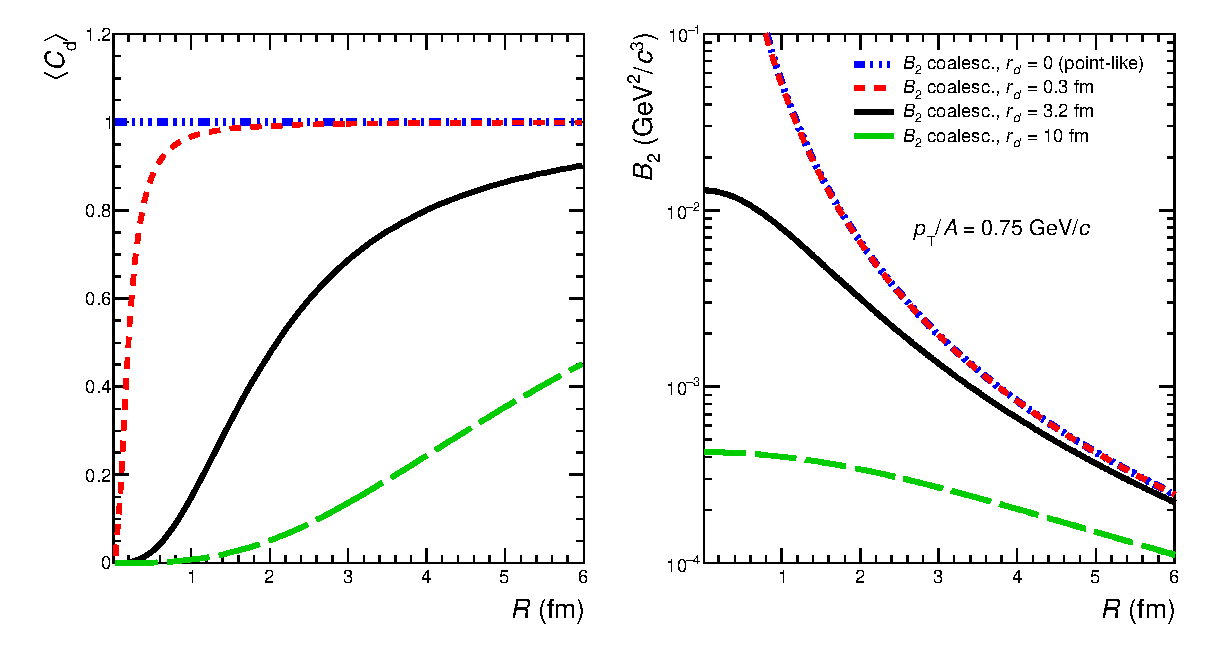
\includegraphics[width=1.0\textwidth]{theory_coalescence_Cd_B2.eps}
\caption{{The quantum mechanical correction factor $\langle C_{d} \rangle$ (left panel, see Eq. \ref{eq:Cdapprox}) and the coalescence parameter \btwo~for deuteron (right panel, see Eq. \ref{eq:B2approx}) as a function of the radius of the source, $R$, calculated assuming a radius of the deuteron $\dradius = 0, 0.3, 3.2$ and $10$ fm.}}
\label{fig:radiusDependence}
\end{center}
\end{figure}

Following the approach and discussion presented in~\cite{Blum:2017qnn}, Eq.~\ref{eq:Cd} may be generalised as 

\begin{equation}
\langle C_{A} \rangle = \prod_{i=1,2,3} \left(1 + \frac{r^2}{4R_{i}^2} \right)^{-\frac{1}{2}(A-1)}
\label{eq:CA_general}
\end{equation}
%
for mass number $A$ and the radii $R_{i}$ which describe the volume of the emitting source.
Similarly, the coalescence parameter \bA~for a nucleus with mass number $A$ and spin $J_{A}$ is generalised in \cite{Scheibl:1998tk} as
\begin{equation}
\bA = \frac{2J_{A} +1}{2^{A}}\frac{1}{\sqrt{A}}  \langle C_{A} \rangle \left( \frac{(2\pi)^{3/2}} {m_{T}\prod_{i=1,2,3} R_{i}} \right)^{A-1}.
\label{eq:BA_general}
\end{equation}
In particular, for the case of \hethree~with $A=3$ and $J=1/2$, Eq. \ref{eq:BA_general} becomes Eq. 9 presented in \cite{Blum:2017qnn}:
\begin{equation}
\bthree = \frac{(2\pi)^{3}}{4\sqrt{3}} \langle C_{3} \rangle (m_{T}\prod_{i=1,2,3} R_{i})^{-2}
\label{eq:B3}
\end{equation}
 
 where
 
 \begin{equation}
\langle C_{3} \rangle \approx \prod_{i=1,2,3} \left(1 + \frac{r_{3}^2}{4R_{i}^2} \right)^{-1}.
\label{eq:C3}
\end{equation}
 

\subsection{Source volume}
\label{SecSourceVolume}
As in \cite{Scheibl:1998tk}, we identify the source volume as the effective sub-volume of the whole system which is governed by the homogeneity length of the interacting nucleons. In addition, the same authors claim that this volume is experimentally accessible with Hanbury-Brown-Twiss (HBT) interferometry. 
The experimental results are typically obtained following the Bertsch-Pratt (BP) parameterisation ($R_{out}, R_{side}, R_{long}$), while the coalescence model described in Section \ref{sec:coalescence} expresses the volume in terms of the Yano-Koonin-Podgoretskii (YKP) parameterisation. As discussed in Appendix \ref{appendix1}, we identify $\rperp = R_{side}$ and $\rpar = R_{long}$, thus $R = (\rperp^{2}\rpar)^{1/3} \approx (R_{side}^{2}R_{long})^{1/3}$.

Experimentally, the size of the effective volume can be controlled by selecting different collision geometries, i.e. different centrality classes \cite{Abelev:2013qoq}. In heavy-ion collisions the HBT radii are known to scale with the cubic root of the average charged particle multiplicity density \avdNdeta$^{1/3}$ \cite{Adam:2015vna}, and to depend on the pair average transverse momentum $\langle k_{\mathrm{T}}\rangle$ \cite{Aamodt:2011mr}. In the following, we make the simplifying assumption that the scaling with \avdNdeta$^{1/3}$ holds across collision systems, which is approximately fulfilled in data \cite{Adam:2015pya}. In contrast to \cite{Blum:2017qnn}, we therefore do not explicitly use the measured HBT radii in our study, but we derive the radii from the measured \avdNdeta~according to the following relation:

\begin{equation}
R = a \avdNdeta^{1/3} + b
\label{eq:radiusParameterisation}
\end{equation}

The coefficients, $a = 0.339$ and $b = 0.128$, have been determined by fitting linearly the ALICE data, and the parameterisation is reported in Fig. \ref{fig:radiiparam}. 
These values are consistent with the radius from kaon femtoscopy for $m_{\mathrm{T}} \approx 1$ \GeVc~in low-multiplicity pp collisions \cite{Abelev:2012sq} and the radius from pion femtoscopy in high-multiplicity \PbPb~collisions at the highest available $k_{\mathrm{T}} \approx 0.8$ \GeVc~\cite{Adam:2015vna}. 
The highest $k_{\mathrm{T}}$ bin was chosen as it corresponds in $m_{\mathrm{T}}$ to the lowest transverse momentum per nucleon (\pt/$A \approx 0.8$ \GeVc) accessible by ALICE for the measurement of nuclei production. 
Ideally, one would use the proton femtoscopic radii for such study, but given that these measurements are not  available in all collision systems, we assume that $m_{\mathrm{T}}$-scaling holds for HBT radii \cite{Adam:2015vja}.

\begin{figure}[htbp]
\begin{center}
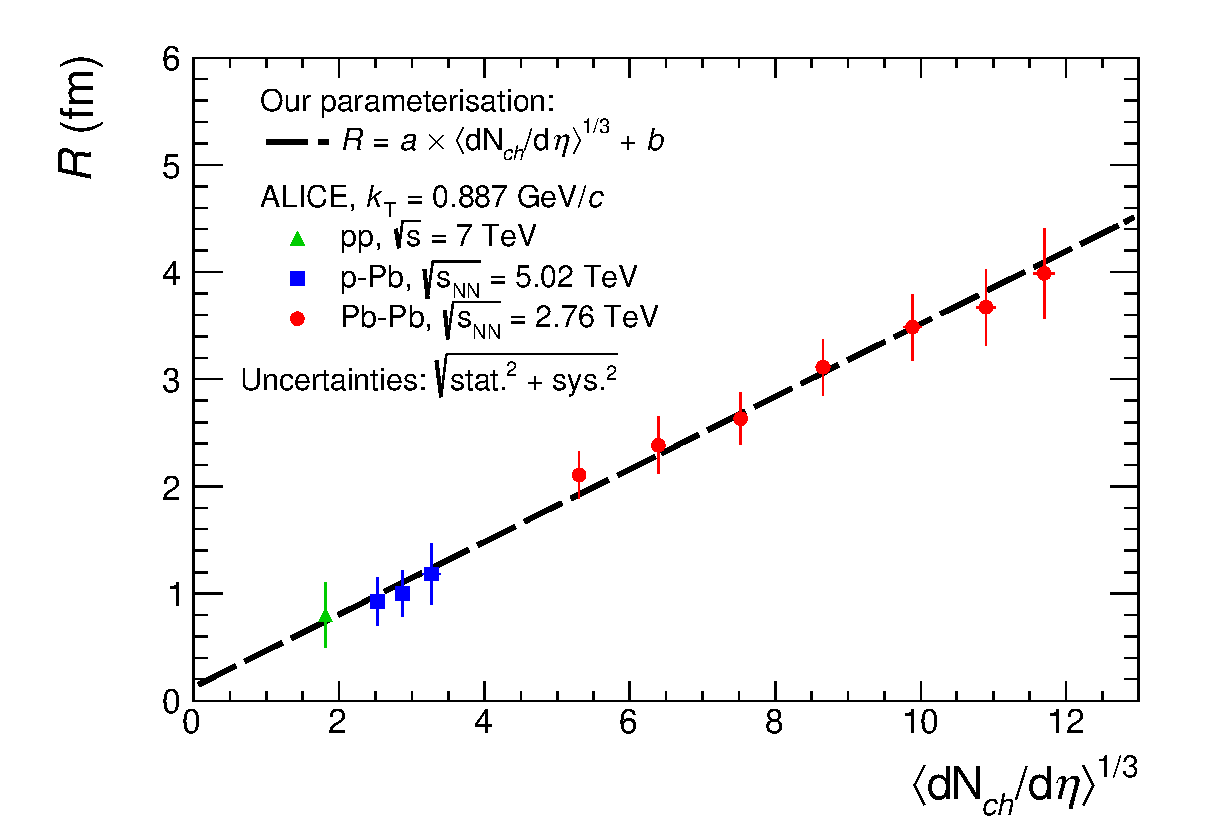
\includegraphics[width=0.6\textwidth]{HbtRadiusParam.eps}
\caption{Parameterisation of the dependence of the source radius on multiplicity assumed in this paper, compared to HBT data from \cite{Adam:2015vna, Abelev:2012sq}.}
\label{fig:radiiparam}
\end{center}
\end{figure}


- excess binding energy needs to be released to the system to make coalescence work


\section{Statistical-thermal approach and blast-wave}\label{sec:thermal}

In the statistical-thermal approach, the yields (d$N$/d$y$) of light anti- and hyper-nuclei are very sensitive to the chemical freeze-out temperature $T_{chem}$ due to their large mass $m$ and approximately scale as d$N$/d$y \propto \exp(-m/T_{chem})$. As a matter of fact, the chemical freeze-out temperature defines the only scale in this model, since at the LHC the chemical potentials which ensure the conservation of baryon number ($\mu_{B}$), strangeness ($\mu_{S}$), and electric charge ($\mu_{Q}$) are negligible.
In contrast to the coalescence approach, the current implementations~\cite{} of the statistical-thermal model provide only \pt-integrated yields and not the full hadron spectra. 
In order to fill this gap, and for the purposes of this exercise, \pt~spectra have been modeled using a blast-wave~\cite{} parameterization. When extracting the predicted spectrum for a given particle species (proton, $\Lambda$, deuteron, \hethree), the parameters of the blast-wave (average radial flow velocity $\langle\beta_{T}\rangle$, kinetic freeze-out temperature $T_{kin}$, and velocity profile $n$) are fixed to the values obtained from the simultaneous fit of the pion, kaon and proton spectra measured in each collision system and multiplicity event class by ALICE~\cite{}. 
The normalisation is fixed using the \pt-integrated deuteron-to-pion ratio and \hethree-to-pion ratio predicted by the GSI-Heidelberg model with $T_{chem} = 156$ MeV, multiplied by the pion yield measured by ALICE~\cite{}. 
This choice is motivated by the fact that the measured proton yield is seen to be slightly underestimated by the thermal model predictions at the LHC~\cite{}.
In the case of hyper-triton, a slightly different procedure is chosen, namely the normalisation for \hthreelambda~is extracted from the statistical-thermal model prediction of the strangeness population factor $S_{3}$ multiplied by the measured $\Lambda/p$ ratio \cite{} and the measured \hethree~yield \cite{}. Based on the thus obtained spectra, we calculate the corresponding coalescence parameters for a given \pt/A and compare it with coalescence expectations. Because we use experimental data to constrain the blast-wave prediction as well as the normalisation, and because such data are provided for given centrality/multiplicity classes, we use the corresponding \avdNdeta~in the same class to estimate the system radius based on the parameterisation discussed in Sec.~\ref{SecSourceVolume}. 
In contrast to the coalescence approach which explicitly depends on the size of the produced object with respect to the system size, the object size does not enter in the formulation of the blast-wave model, which as a simplified hydrodynamic model treats the system based as a continuum and is not particle based. The thermal model on the other hand, implements eigenvolume corrections where the object radius is fixed as an external parameter ($r=0.3$~fm in the case of baryons for the GSI-Heidelberg prediction used here). We refer to the literature for the extensive discussions on the validity of the eigenvolume correction for light anti- and hyper-nuclei~\cite{Volodya} and the relation with the possible production of these objects as compact quark bags~\cite{Andronic:2017}.



\section{Comparison with experimental data}\label{sec:comparison}

Data on anti- and hyper-nuclei production at LHC energies and different collision systems have been released by the ALICE Collaboration in recent years \cite{}. 
In Fig. \ref{} we compare the coalescence parameter \btwo~from the coalescence model (see Eqs.~\ref{eq:B2cd} and \ref{eq:B2approx}, with $r_{d} = 3.2$ fm) with the ALICE data.  
First, the parameterisation of the system radius fitted to the HBT data as described in Sec.~\ref{SecSourceVolume} is used to map the \avdNdeta~to the source size (datapoints shown with \textcolor{red}{empty markers}).
We notice already at this point that the coalescence volume from our extracted parameterisation of the HBT radii leads to discrepancies with respect to the curve from the coalescence calculation, and in particular, we notice that the model would require a larger radius for a given value of \btwo.
Therefore, in a second step the radius is tuned such that the data points for (anti-) deuterons fall onto the coalescence prediction (solid markers). We find that the parameters of Eq.~\ref{eq:radiusParameterisation} turn out to be \textcolor{red}{$a = xxx$ and $b = yyy$}. 
With this second parameterisation, we investigate also the agreement of the model with the measured coalescence parameter \bthree. As shown in Fig.~\ref{}, also in the case of \bthree, a tension between the model and the data is found which persists with both parameterisations.
It is also noteworthy that any change of the radii parameterisation would result in a shift along the x axis of both \btwo~and \bthree~data points in the same way, while the theoretical coalescence curve would not be affected. 
 
- discuss sensitivity to the choice of the kT for the radii parameterisation.

- add a plot with different radii for hyper-triton from 10fm to 3fm

- add a plot for A=4

- add a plot for the X(3872)???? --> Look at the ExHic and Maiani rebuttal


\subsection{(Anti-)nuclei with $A$ = 2, 3, 4}
\subsection{(Anti-)hyper-nuclei}
- cite Che Ming Ko \cite{Zhang:2018euf} 
\section{Projections for the LHC Run 3 and 4}\label{sec:projections}

\section{Summary and conclusions}

We conclude that (c.) appears unlikely, thus leaving (b.) as a viable option, at least with our present knowledge of the hypertriton size.



%%%%%%%%APPENDIX
\begin{appendix}
\section{HBT radii in Bertsch-Pratt and Yano-Koonin-Podgoretskii parameterisation for comparison with coalescence models}
The results of HBT analyses are typically presented in either the Bertsch-Pratt ($R_{out}$, $R_{sside}$, $R_{long}$) or the Yano-Koonin-Podgoretskii ($R_{\perp}$, $R_{0}$, $R_{\parallel}$) parameterization. The ALICE HBT results \cite{Aamodt:2011mr, Adam:2015pwa} are given in the Bertsch-Pratt convention, whereas the coalescence parameter is derived in \cite{Scheibl:1998tk} by expressing the dependence on the volume in terms of the Yano-Koonin-Podgoretskii (YKP) parameterisation. 
The transformation between the two parameterisations is best presented in~\cite{Wiedemann:1999qn} in the equations (W 3.48) to (W 3.52)\footnote{The equations in~\cite{Wiedemann:1999qn} are denoted as (W...) in order to distinguish them from the equations presented in this paper.}:

\begin{eqnarray}
R_{side}^{2}    &=& R_{\perp}^{2}  \;, \\
R_{diff}^{2} &=& R_{out}^{2} -  R_{side}^{2} = \beta_{\perp}^2 \gamma^2 (R_{0}^2 + v^2R_{\parallel}^2) \;, \\
R_{long}^{2}     &=& (1 - \beta_l^2) R_{\parallel}^2 + \gamma^2 (\beta_l - v)^2 (R_{0}^2 + v^2R_{\parallel}^2) \;, \\
R_{ol}^{2}   &=& \beta_{\perp} (-\beta_l R_{\parallel}^{2} +  \gamma^2 (\beta_l - v)(R_{0}^2 + v^2R_{\parallel}^2)) \,.
\end{eqnarray}
%
We immediately identify that $R_{\perp}^2$ can be identified with $R_{side}^{2}$. Following the reasoning and the nomenclature in~\cite{Wiedemann:1999qn} (W 3.52-3.53), the above equations can be inverted and $R_{\parallel}^{2}$ can be expressed as 
%
\begin{eqnarray}
R_{\parallel}^{2} &=& B  - v \cdot C \;, \\
                          &=& R_{long}^2 - 2{\beta_l \over \beta_\perp}  R_{ol}^2 + {\beta_l^2 \over \beta_\perp^2} R_{diff}^2 
                          - v \cdot \Bigl(-{1 \over \beta_\perp } R_{ol}^2 + {\beta_l \over \beta_\perp^2} R_{diff}^2  \Bigr) \; .
\end{eqnarray}
%
As it turns out all corrections which are subtracted from $R_{long}^{2}$ can be neglected. First, we notice that the cross term $R_{ol}$ vanishes if the measured fireball is longitudinally boost-invariant, which is a valid approximation for the rapidity ranges studied here. The remaining terms are all proportional to $\beta_l$, which is also $\beta_l = 0$ by definition of the rest frame for a longitudinally-boosted invariant system. In summary, we can consider $R_{\perp} = R_{side}$ and $R_{\parallel}=R_{long}$ for the present study.
\end{appendix}


%%%%% acknowledgements
\newenvironment{acknowledgement}{\relax}{\relax}
\begin{acknowledgement}
\section*{Acknowledgements}
We thank U. Heinz for the useful discussions and the clarification on the equivalence of the Bertsch-Pratt and Yano-Koonin-Podgoretskii parameterisations of the HBT radii.
The authors would like to thank themselves for the auto-critics.

\end{acknowledgement}



\bibliographystyle{utphys} 	
\bibliography{NucleiB2}




\end{document}




%%
%% End of file.
